\documentclass[../main.tex]{subfiles}
\begin{document} \label{chapter_hmms}
In this chapter, we continue delving into the pipeline proposed in section \ref{general_pipeline}. Having extracted formant trajectories, we are now interested in building a more abstract structure that summarises their shape and content. This reflects the need to measure the similarity of the trajectories \emph{as a symbol}, rather than as discrete sequences of varying length. Once any such structure has been trained, a similarity measure can be used to create a distance matrix, which serves as input to some of the relational structure building algorithms described in section \ref{algorithms_review}.
\par Therefore, this chapter is divided in three parts: sections \ref{section_kde} and \ref{section_hmm} concern Kernel Density Estimation and Hidden Markov Models, which are related to the abstract structures discussed above; then, section \ref{section_similarity} presents similarity measures between probability densities and between Hidden Markov Models; finally, section \ref{section_hierarchical} reviews hierarchical clustering for building arborescent relational structures.
\par Although this chapter only gives a theoretical account of the techniques to further characterise birdsong, these form a key component to describe how they relate to birdsong. This discussion is saved for chapter \ref{chapter_account}, in which we give a full description of how each of these techniques can be combined with formant trajectories to characterise birdsong.

\section{Kernel density estimation} \label{section_kde}
In this section, we describe Kernel Density Estimation, which is a technique useful to fit probability distributions to data. We focus the discussion on the unidimensional case, and refer the reader to the cited works for the multivariate case. 
\par Given a continuous distribution $F(x)$ with density $\frac{d}{dx}F(x) = f(x)$, the goal is to estimate $f(x)$ from a finite sample $X = \{x_1, x_2, ..., x_N\}$ \cite{Hansen2009}, assuming they are independently and identically distributed. 
\par The easiest approach to build probability distributions is to use histograms. Histograms are built by dividing an interval into $M$ bins of not-necessarily-equal width, counting how many points fall within each bin, and normalising these quantities so that it becomes a probability distribution. In other words, we first generate a vector $B = (b_0, b_1, b_2, ..., b_M)$, where $b_{i+1} - b_i = w_i, 0 < i \leq M$ is the width of bin $i$ and the $b_i$ are called endpoints. Then, the vector 
\begin{align*}
\V{H} &= (H_i)\\
H_i &= \frac{1}{N}\sum_{j=1}^{N}\frac{\mathbb{I}( b_{i} < x_j \leq b_{i+1})}{w_i}, \forall i \leq M
\end{align*}
\par is the histogram corresponding to the dataset $X$ for the given endpoints.
\par There are two issues with the proposal above: on one hand, the histogram function is not smooth, i.e. we are prone to see discontinuities at the edges of each bin; on the other hand, each histogram depends heavily on its endpoints, both in terms of the width of each bin, and in terms of \emph{where} they are located \cite{Duong2004}. This results in having radically different histograms for each selection of endpoints, as can be seen in figure \ref{fig_histograms}.
\begin{figure}[t]
\centering
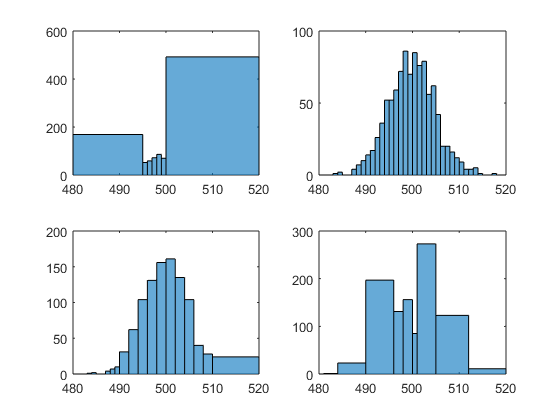
\includegraphics[width=\textwidth]{histograms}
\caption{Four histograms over the same data, with different bin edges in each subplot.}
\label{fig_histograms}
\end{figure}
\par Therefore, we are interested in proposing a method that overcomes these issues. To do so, we first remark the following: consider the set of uniform distributions given by $\{\mathcal{U}_i = \mathcal{U}(b_{i}, b_{i+1})\}$. This distribution covers a range of length $w_i = b_{i+1}-b_i$ and is centered in $c_i = \frac{b_{i+1}+b_i}{2}$.  Let $h_i = \frac{w_i}{2}$ and notice that anytime $\abs{x_j - c_i} \leq h_i$, or equivalently,
\begin{align*}
\abs{\frac{x_j - c_i}{h_i}} \leq 1
\end{align*}
\par then an instance of the uniform distribution $\mathcal{U}_i(x) = \frac{\mathbb{I}(b_i < x \leq b_{i+1})}{2h_i}$ is ``stacked" over $c_i$. To summarise, we can conclude that the histogram probability distribution can be modelled equivalently as:
\begin{align*}
p_H(x) = \frac{1}{N}\sum_{i=1}^M\frac{1}{2h_i}\mathbb{I}\left(\abs{\frac{x - c_i}{h_i}} \leq 1\right)
\end{align*}
\par In other words, we have an asset of $N$ uniform distributions centered at each $c_i$; by additivity of integration, the total area under these distributions is equal to $N$, and thus we just have to normalise by dividing over $N$ to make this linear combination a new probability distribution. Now, assume that we let each uniform distribution $\mathcal{U}_i$ have the same width, and that we center each uniform distribution at each $x_j \in X$, i.e. now we have $N$ overlapping bins. Then, the expression above becomes:
\begin{align*}
p_{H}(x) &= \frac{1}{N}\sum_{j=1}^N\frac{1}{2h}\mathbb{I}\left(\abs{\frac{x - x_j}{h}} \leq 1\right)\\
&= \frac{1}{Nh}\sum_{j=1}^NK_u(\abs{\frac{x - x_j}{h}}),\\
K_u(x) &= \left\{
     \begin{array}{lr}
      \frac{1}{2} & \abs{x} \leq 1 \\
      0 & \text{otherwise} 
     \end{array}
   \right.
\end{align*}
\par This function does no longer look like a histogram, but rather like a staircase pyramid, as shown in figure \ref{fig_hist2}. Moreover, we also notice that we have transformed our original expression so as to make it depend on a very well known function, the uniform kernel $K_u$ \cite{Hansen2009}. 
\begin{figure}[t]
\centering
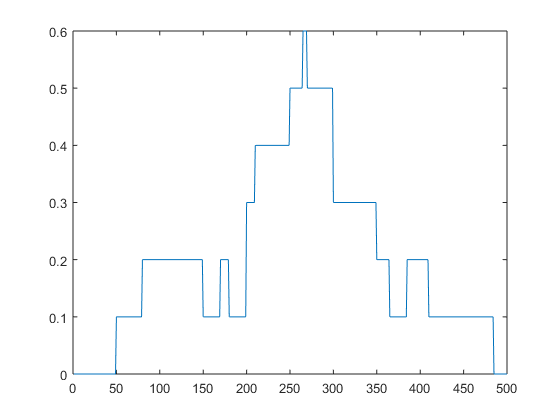
\includegraphics[width=80mm]{histogram2}
\caption{The probability distribution generated by placing uniform distributions of the same width along the $x$ axis, centered around each data point $x_j$.}
\label{fig_hist2}
\end{figure}
\par Although this function does not look smooth yet, we can now use the fact that it depends on the kernel $K_u(x)$, and think of the latter as a brick used to shape the resulting density. We recall that a kernel is any function that integrates to one, i.e. $\int_{-\infty}^\infty K(x)dx = 1$. A non-negative kernel $K$ is one such that $K(x) \geq 0 \forall x$, in which case $K$ is a probability distribution \cite{Hansen2009}.
\par This is the idea behind Kernel Density Estimation: we can approximate the probability density function of a set of points as a weighted linear combination of small ``bricks" (non-negative kernels). 
\begin{align*}
p_K(x) = \frac{1}{Nh}\sum_{i=1}^NK(\abs{\frac{x - x_i}{h}}),\\
\end{align*}
\par Furthermore, instead of using the uniform kernel as we did previously, we can use a smooth kernel and hence (given that the sum $f+g$ of two continuous functions $f, g: \mathbb{R} \rightarrow \mathbb{R}$ is continuous) get back a smooth probability function. Naturally, intervals where there is a greater density of data will have taller bumps in the resulting probability distribution, whereas intervals with scarce data will be assigned a very low probability.  
\par By using a smooth kernel instead of the crispy and flat uniform kernel, we can remove the edges at each endpoint of the histogram's bins and thus get a smooth probability function as a result. However, this still does not solve the issue with the width parameter $h$ (without loss of generality called bandwidth for kernels). The bandwidth $h$ controls the degree of smoothness of the curve, and thus tuning it is crucial in order to get accurate results. The resulting probability function could be oversmoothed, undersmoothed or optimally smoothed, as is depicted in figure \ref{fig_kdebandwidths}, depending on the value of $h$ \cite{Duong2004}.
\begin{figure}[t]
\centering
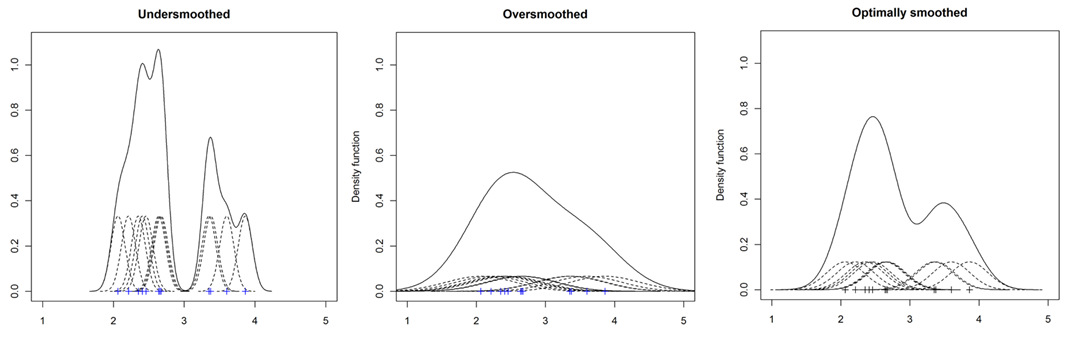
\includegraphics[width=\textwidth]{kdebandwidth}
\caption{Three probability density functions fitted using KDE with Gaussian kernels and different bandwidths. Images retrieved from \cite{Duong2004}.}
\label{fig_kdebandwidths}
\end{figure}
\par One of the most common smooth kernels in the literature is the Gaussian kernel \cite{hastie2008}, given by:
\begin{align*}
K_G(x) = \frac{1}{\sqrt{2\pi}}e^{-\frac{1}{2}x^2}
\end{align*}
\par Its popularity is due not only to its close relationship to the Normal distribution (KDE places small Gaussians centered in each datapoint in this case), but also because there is a rule of thumb on how to set the bandwidth $h$. The details of the derivation for this rule are out of the scope of this work, but can be consulted in \cite{Hansen2009}. In particular, for univariate Gaussians, the optimal bandwidth in the least-squares error sense is given by $h = \hat{\sigma}n^{-1/5}$, where $\hat{\sigma}$ is the standard deviation of the sample $X$.

\section{Hidden Markov Models} \label{section_hmm}
In this section, we describe a useful statistical model to analyse the content and shape of sequences of observations over time: Hidden Markov Models (HMM). Firstly, we define and discuss the purpose of Hidden Markov Models; then, we present Gaussian Mixture Models (GMMs), which are probability distributions capable of modelling subpopulations in a dataset as a weighted combination of Gaussian distributions; next, we introduce the Wishart and Dirichlet distributions, which prove useful in the Bayesian setting; finally, we discuss Variational Inference, a powerful framework that enables us to model uncertainty and train models that take into account our beliefs about the models' parameters.

\subsection{Definition} \label{subsection_defhmms}
In this subsection, we introduce the theory behind Hidden Markov Models and describe the scenarios where they prove to be useful. We first present the more general concept of Markov Chain, which will allow us to introduce HMMs more naturally. 
\par Assume that a system is in a state $s_t$ from a set $Q = \{ q_1, q_2, ..., q_K \}$ at time $t$, and that we observe the system periodically so as to obtain a sequence $\V{s} = \left( s_1, s_2, ..., s_T \right)$, where $s_t \in Q$. Remark that we are able to observe the state of the system, so we confirm what its state is at any time $t$. Furthermore, assume that the state the system reaches at $t+1$, $s_{t+1}$, only depends on where it was one time step before, $s_t$. That is, $s_{t+1}$ is conditional only on $s_{t}$, and does not go further back in time to make a decision. Then, we say that the system satisfies the \emph{Markov property} \cite{Murphy2012}.
\par A Markov Chain models the transition probabilities $p(s_{t+1} \given s_t)$ of a system satisfying the Markov Property. By the product rule, we can model the probability that a given sequence was generated by the system as:
\begin{equation}\label{eq:chain}
p(\V{s}) = p(s_1)\prod_{t=1}^{T-1}p(s_{t+1} \given s_t)
\end{equation}
\par Nevertheless, it is not always true that we are able to observe the state of the system of study. In other words, some systems might have a latent (hidden) Markov process for which we can only obtain a sequence of observations $\V{x} = \left( \V{x}_1, \V{x}_2, ..., \V{x}_T \right)$, but not its associated state sequence $\V{s}$. Because we cannot directly observe what state the system is in, we can only say that a particular observation $\V{x}_t$ is generated by state $\V{s}_t$ with probability $p(\V{x}_t \given \V{s}_t)$ \cite{Murphy2012}. 
\par In this scenario, we can now ask for the probability that the model generated such observations $\V{x}$ and that the underlying Markov Process generated the sequence of states $\V{s}$. This is given by the joint probability $p(\V{x}, \V{s})$, which can be expanded in terms of equation \ref{eq:chain}.
\begin{equation}\label{eq:hmm}
p(\V{x}, \V{s}) = p(\V{s})p(\V{x} \given \V{s}) = p(s_1)\prod_{t=1}^{T-1}p(s_{t+1}\given s_t)\prod_{t=1}^Tp(\V{x}_t \given s_t)
\end{equation} 
\par A Hidden Markov Model is a statistical tool that models the scenario presented above, in which we observe a sequence $\V{x}$ associated to a sequence of latent states $\V{s}$ and then want to infer, for example \cite{Jurafsky2009, Bishop2006}: given a sequence of observations $\V{x}$ and an HMM, what is the sequence of states $\V{s}$ that most likely generated $\V{x}$? Or: given a sequence of observations $\V{x}$ and a sequence of states $\V{s}$, what is the probability $p(\V{x} \given \V{s})$ that $\V{s}$ generated $\V{x}$?  
\par From equation \ref{eq:hmm} we can remark three key elements \cite{Ghahramani2001}: the factor $p(s_1)$ is the probability of starting the process in state $q_k \in Q$, and therefore is a associated to a distribution $\pi(q_k)$ over the states $Q$. This is called the \emph{initial state distribution}. Next, the transition probabilities $p(s_{t+1} \given s_t)$ are associated to a Markov chain describing the probabilities $p(q_j \given q_i)$, i.e. going from state $q_j$ to state $q_i$. This is called the \emph{transition model}, and is described by a matrix $A$ with entries $a_{i,j} = p(q_j \given q_i)$. Finally, the observations are linked to a distribution called the \emph{observation model}, with parameters $\phi$. 
\par An HMM is fully characterised (up to a permutation of states) by these three parameters $\theta = (\phi, B, \pi)$. Furthermore, the observations analysed by an HMM can be continuous or discrete, and an HMM is then called continuous or discrete HMM accordingly \cite{Jurafsky2009}. In our discussion, we will focus on continuous observations. More details are given in subsection \ref{subsection_gmm}.
\par Remark that for every HMM with $K$ states, there exist $K!$ equivalent HMMs that can be generated by permuting the identities of the HMM's states. This problem is called \emph{identifiability} \cite{Bishop2006}, and will play an important role when we define a metric between HMMs. 

\subsection{Gaussian Mixture Models}\label{subsection_gmm}
Consider the scenario depicted in subsection \ref{subsection_defhmms}, in which we analyse a sequence of observations $\V{x}$ associated to a sequence of latent states $\V{s}$. Assume that we drop the structure of the sequence, and instead focus on the \emph{content} of the observations in $\V{x}$, i.e. we focus on the associated set $\mathcal{X} = \{\V{x}_1, \V{x}_2, ..., \V{x}_T\}$ (without loss of generality, and letting each $\V{x}_t$ still be identifiable). Since each $\V{x}_t$ is still associated with a state $s_t$, we could think of the subsets $\mathcal{X}_i = \{\V{x}_t \mid \V{x}_t$ is associated with $q_i \}$ as a partition of $\mathcal{X}$ for each $\mathcal{S} = \{s_t\}$.
\par We can also think of each $\mathcal{X}_i$ as a subpopulation of $\mathcal{X}$. Furthermore, assume that all the elements $\V{x}_t^{(i)}$ of a single subpopulation $\mathcal{X}_i$ are drawn from the same probability distribution $p_i(\V{x}_t \given \theta)$, where $\theta$ parametrises $p_i$. Then, the probability distribution from which the whole set $\mathcal{X}$ was drawn from can be seen as a convex combination of the family $\{p_i\}$:
\begin{equation} \label{eq:mixmod}
p(\V{x} \given \theta ) = \sum_{i=1}^K\pi p_i(\V{x} \given \theta)
\end{equation}
where the $\pi_i$ are called weights and satisfy  $0 \leq \pi_i \leq 1 \forall i, \sum_i \pi_i = 1$. 
\par This is what we call a \emph{mixture model} \cite{Murphy2012}. In particular, a Gaussian Mixture Model is one in which we let all $p_i$ be normal distributions, i.e. $p_i(\V{x} \given \theta) = \mathcal{N}(\V{\mu}_i, \Sigma_i) \forall i$.
\par GMMs allow us to study subpopulations independently (by analysing each $p_i$ individually) or as a group (by considering the convex combination). This makes them a suitable choice for an emission model that generates continuous observations \cite{Jurafsky2009}. A depiction of GMMs can be seen in figure \ref{fig_gmm}.
\begin{figure}[t]
\centering
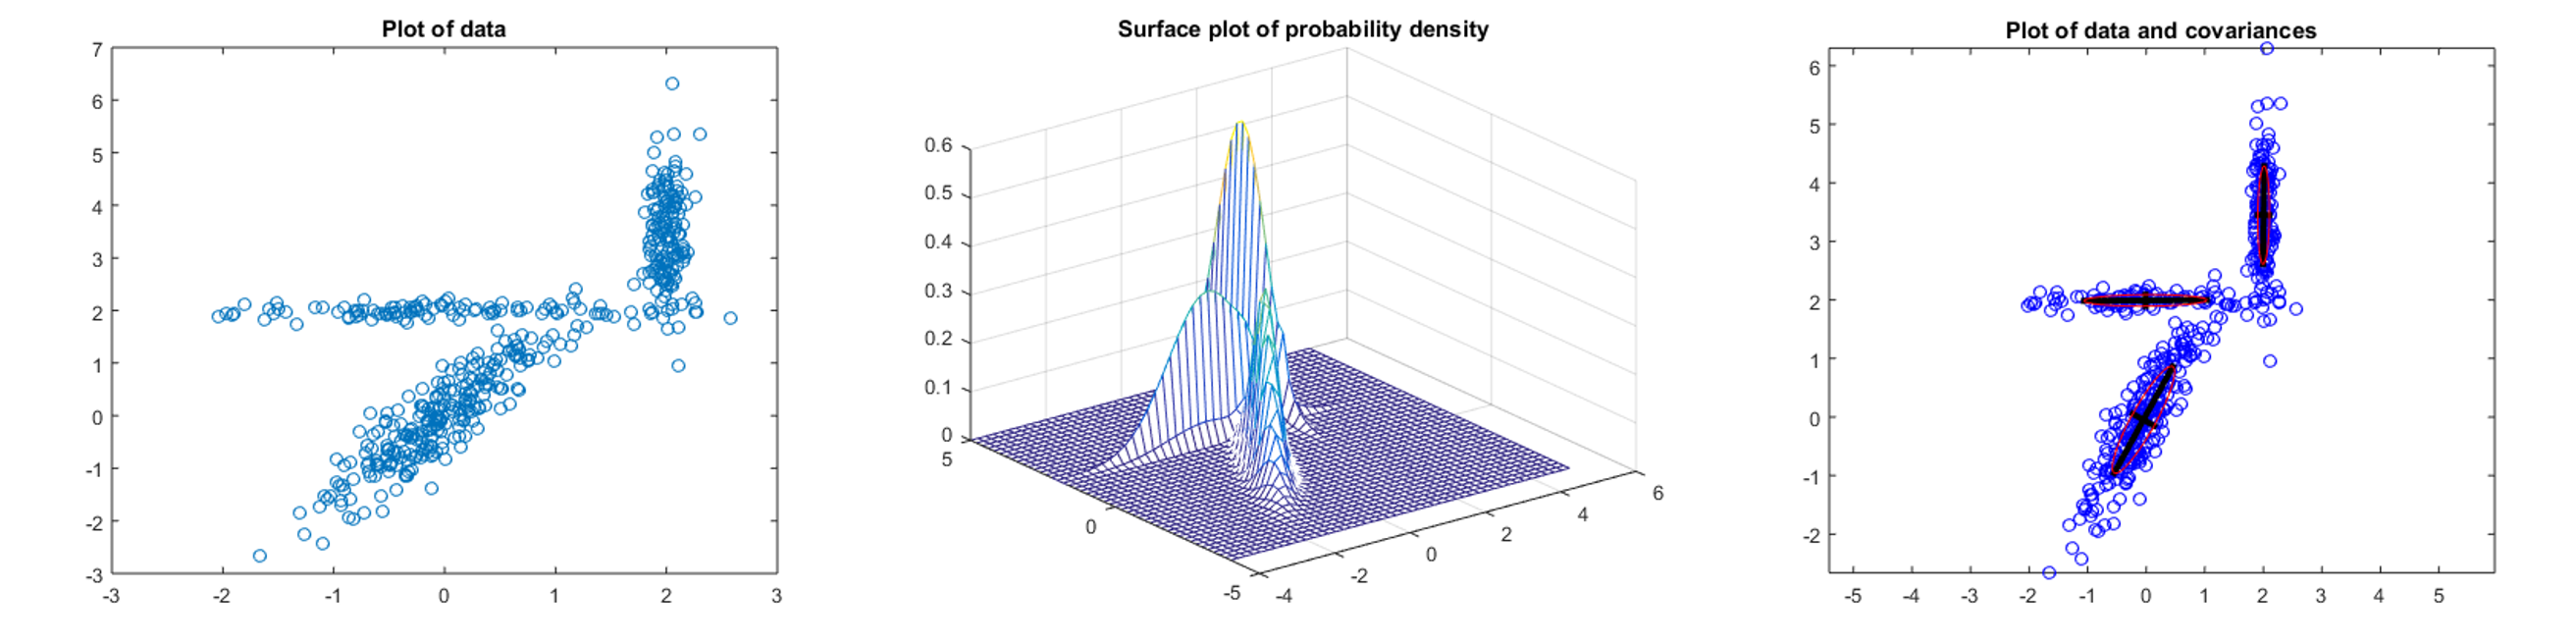
\includegraphics[width=\textwidth]{gmm}
\caption{Left: data drawn from three normal distributions. Center: GMM with three components fitting the data. Right: level curve of each GMM component over the subpopulation it representes. These images were generated using the NETLAB toolbox.}
\label{fig_gmm}
\end{figure}

\subsection{Dirichlet and Wishart distributions} \label{subsection_dirwish}
In this section, we introduce two probability distributions relevant in the Variational Bayes approaches described in subsection \ref{subsection_model}: the Dirichlet and the Wishart distributions. 
\par The Dirichlet distribution is a multivariate generalisation of the Beta distribution, and is only defined over the probability simplex \cite{Murphy2012}, given by:
\begin{align*}
S_K = \left\{\V{x} : 0 \leq x_k \leq 1, \sum_{k=1}^Kx_k = 1\right\}
\end{align*}
Its density function is given by:
\begin{equation} \label{eq:dirichlet}
\text{Dir}(\V{x} \given \V{\alpha}) = \frac{1}{B(\V{\alpha})} \prod_{k=1}^Kx_k^{\alpha_k-1}\mathbb{I}(\V{x}\in S_K)
\end{equation}
Where $B(\V{\alpha})$ is the normalisation constant, given by:
\begin{equation}
B(\V{\alpha}) = \frac{\Pi_{k=1}^K\Gamma(\alpha_k)}{\Gamma(\sum_{k=1}^K\alpha_k)}
\end{equation}
And $\Gamma(t)$ is the Gamma function, defined as:
\begin{equation}\label{eq:gamma}
\Gamma(t) = \int_0^\infty x^{t-1}e^{-x}dt
\end{equation}
Remark that the probability simplex is a set of tuples that form a Categorical distribution with $K$ possible outcomes. Additionally, these tuples can also be seen as the parameters of a Multinomial distribution. In other words, the Dirichlet can be seen as a distribution over the Categorical and Multinomial distributions.
\par The second distribution we discuss in this subsection is the Wishart distribution. It is a generalisation of the Gamma distribution to positive-definite matrices. 
\begin{definition}{Positive-definite matrix.} \label{def_pdmatrix}
A symmetric matrix $A \in \mathbb{R}^{n\times n}$ is said to be positive-definite if for all vectors $\V{z} \in \mathbb{R}^n$ the following holds:
\begin{align*}
\V{z}A\V{z}^T > 0
\end{align*}
\end{definition}
\par The Wishart distribution is often used to model uncertainty of covariance matrices $\Sigma$ and their inverses, precision matrices $\Lambda = \Sigma^{-1}$ \cite{Murphy2012}. Its probability density is given by:
\begin{align*}
\text{Wi}(\Lambda \given S, \upsilon) = \frac{1}{Z_{\text{Wi}}} \abs{\Lambda}^{(\upsilon -D -1)/2}\exp{\bigg(-\frac{1}{2}\text{tr}(\Lambda S^{-1})\bigg)}
\end{align*}
Where $\upsilon$ is called the \emph{degrees of freedom}, $S$ is called the scale matrix, tr$(A)$ denotes the trace of matrix $A$, and $Z_{\text{Wi}}$ is the normalisation constant given by:
\begin{align*}
Z_{\text{Wi}} &= 2^{\upsilon D / 2}\Gamma_D(\upsilon/2)\abs{S}^{\upsilon/2}
\end{align*}
For $\upsilon > D-1$, and $\Gamma_D(x)$ is the $D$-dimensional multivariate Gamma function, defined as:
\begin{align*}
\Gamma_D(x) = \pi^{D(D-1)/4}\prod_{i=1}^D\Gamma(x+(i-1)/2)
\end{align*}
There is an interesting relationship between the Wishart and the multivariate normal distribution \cite{Nydick2012}. Let $\V{x}_1, \V{x}_2, ..., \V{x}_N$ be $p$-dimensional samples with $\V{x}_i \sim \mathcal{N}(0, \Sigma)$. Furthermore, let $X \in \mathbb{R}^{n \times p}$ be the matrix obtained by stacking the elements $\V{x}_i$ as rows. Then, $S = X^TX \sim \text{Wi}_p(\Sigma, n)$. 

\subsection{Training and model selection} \label{subsection_model}
Given the description of HMMs from subsection \ref{subsection_defhmms}, two questions arise naturally: first, how do we choose the number of states $K$ the HMM should have? And second: given a sequence $\V{x}$, how do we \emph{train} an HMM, i.e. how do we find the optimal values for $(A, \phi, \pi)$?
\par Until recently, $K$ was typically chosen by careful study of the field of application. For example, in Human Speech Recognition, $K$ could correspond to the number of phonemes that exist in the target language \cite{Jurafsky2009}. In birdsong recognition, states would correspond to birdsong syllables (like those described in section \ref{birdsong_review}). Additionally, $K$ could also be chosen by training several HMM's with a different value of $K$ \cite{Siddiqi2007,Rezek2005}, and then choosing the one with the best performance under a defined metric.
\par However, these approaches have some disadvantages: on one hand, we need the knowledge of experts from the field of application (e.g. an ornithologist that knows how many syllables a particular species is able to sing); additionally, it also makes HMM comparison less clear: what if two HMMs study the same kind of objects, but differ in number of states (e.g. if we study two different bird species, but each sings a different number of syllables, how do we compare them without losing information?); finally, it is a very expensive procedure, since the time spent training and testing HMMs grows linearly as the number of states becomes larger.
\par Nevertheless, with the advent of Variational Bayes approaches, the number of states is now frequently left to the algorithm to decide. Variational Bayes (VB) approaches have the advantage of \emph{using only the number of states they need to use}, i.e. we only need to give an upper bound on how many states an HMM may end up using, and (under specific circumstances) the VB algorithm will adjust to use only the ones it requires, as has been presented in \cite{Rezek2005}.
\par VB algorithms are useful for training statistical models with latent variables, such as HMMs. Previously, HMMs were frequently trained using the Baum-Welch algorithm, which is an adaptation of the more general Expectation-Maximisation (EM) algorithm \cite{Ghahramani2001}. However, HMMs can also be trained by a VB approach to the EM algorithm. Although full details of the algorithm are outside the scope of this project, some key points will be given below and the reader is referred to \cite{Beal2001,Rezek2005,MacKay1997} for further detail.
\par Variational Bayes Inference is a direct application of the calculus of variations, which is an area in mathematics that studies functionals. Formally, functionals are mappings from a vector space to its underlying scalar field \cite{Bishop2006}. However, for the purpose of this project, we will focus only on functionals from the vector space of continuous real functions into the real numbers $\mathbb{R}$. 
\par An example of a functional is the entropy of a continuous random variable $x$ with probability distribution $p(x)$ \cite{Bishop2006}, given by:
\begin{align*}
H \big[ x \big] = - \int p(x) \log{p(x)} dx
\end{align*}
\par The entropy function is a functional because it acts as a rule mapping a (probability density) function into a real number (the entropy itself).
\par The main idea behind the Bayesian approach is to model uncertainty rather than assuming fixed models. In other words, whereas approaches such as Maximum A Posteriori (MAP) and Maximum Likelihood Estimation (MLE) assume that a model $m$'s parameters $\theta$ are a single fixed point that explains data, the Bayesian approach assumes that parameters are uncertain (a probability distribution) about which we have \emph{beliefs} that change as we see fixed data \cite{Genovese2004}. 
\par More formally, the Bayesian approach seeks to maximise the posterior (i.e. given the data) distribution \cite{Beal2003}:
\begin{equation}\label{eq:bayes_posterior}
p(\theta \given \V{x}, m) = \frac{p(\V{x} \given \theta, m)p(\theta \given m)}{p(\V{x} \given m)}
\end{equation}
\par The equation above holds by Bayes' theorem. The factor $p(\V{x} \given \theta, m)$ is called the likelihood, the prior distribution is $p(\theta \given m)$ and $p(\V{x} \given m)$ is called the marginal likelihood \cite{Beal2003}. Remark that the prior distribution represents our beliefs \emph{before} seeing the data, i.e. the knowledge that we have acquired from the past regarding the behaviour of each parameter \cite{Murphy2012}.
\par The following discussion is based on \cite{Ghahramani2001,Beal2003}. Consider the log-marginal distribution $\log{p(\V{x} \given m)}$ for a model with latent variables. Notice that it can be marginalised by introducing a distribution over the model's latent variables $\V{s}$ and the parameters $\theta$:
\begin{align*}\label{eq:marginal}
\log{p(\V{x} \given m)} &= \log{\int\int p(\V{x}, \V{s}, \theta \given m) d\V{x} d\theta}\\
&= \log{\int\int \frac{q(\V{s}, \theta)}{q(\V{s}, \theta)}p(\V{x}, \V{s}, \theta \given m) d\V{x} d\theta}
\end{align*}
and by Jensen's inequality:
\begin{equation*}\label{eq:jensen}
\log{p(\V{x} \given m)} \geq  \int\int q(\V{s}, \theta)\log{\frac{p(\V{x}, \V{s}, \theta \given m)}{q(\V{s}, \theta)}} d\V{x} d\theta
\end{equation*}
Maximising this lower bound with respect to the free distribution $q(\V{s}, \theta)$ yields $q(\V{s}, \theta) = p(\V{s}, \theta \given \V{x}, m)$, i.e. the posterior distribution. Now assume that we can factorise $q(\V{s}, \theta) \approx q_{\V{s}}(\V{s})q_{\theta}(\theta)$. Then:
\begin{align*}
\log{p(\V{x} \given m)} &\geq  \int\int q_{\V{s}}(\V{s})q_{\theta}(\theta)\log{\frac{p(\V{x}, \V{s}, \theta \given m)}{q_{\V{s}}(\V{s})q_{\theta}(\theta)}} d\V{x} d\theta \\
 &= \mathcal{F}_m(q_{\V{s}}(\V{s}), q_{\theta}(\theta), \V{x})
\end{align*}
Remark that $F_m$ is a functional. Using calculus of variations, we can optimise $F_m$ with respect to $q_{\V{s}}(\V{s})q_{\theta}(\theta)$ simultaneously and come up with alternating update equations:
\begin{align*}
q_{\V{s}}^{(t+1)}(\V{s}) &\propto \exp{ \bigg[ \int \log{p(\V{x}, \V{s} \given \theta, m)} q_\theta^t(\theta) d\theta \bigg] } \\
q_{\theta}^{(t+1)}(\theta) &\propto p(\theta \given m) \exp{\bigg[ \int \log{p(\V{x}, \V{s} \given \theta, m)} q_{\V{s}}^{t+1}(\V{s}))d\V{s} \bigg]}
\end{align*}
Furthermore, it can be proved that the following holds:
\begin{align*}
\log{p(\V{x} \given m)} - \mathcal{F}_m(q_{\V{s}}(\V{s}), q_{\theta}(\theta), \V{x}) &= \int\int q_{\V{s}}(\V{s})q_{\theta}(\theta)\log{\frac{q_{\V{s}}(\V{s})q_{\theta}(\theta)}{p(\V{x}, \V{s}, \theta \given m)}} d\V{x} d\theta\\ &= \text{KL}\infdiv{q}{p}
\end{align*}
In other words, finding the distributions $q_\V{s}, q_\theta$ that best approximate the true posterior by maximising $\mathcal{F}_m$ is equivalent to minimising the KL-divergence between the approximation $q(\V{s}, \theta)$ and the true posterior $p(\V{s}, \theta \given \V{x}, m)$ \cite{Ghahramani2003}. This iterative procedure resembles the EM algorithm mentioned earlier in this subsection, in the sense that we make alternating updates to estimate our beliefs about the parameters.
\par Additionally, notice that the update equation for $q_{\theta}^{(t+1)}(\theta)$ makes use of the prior distribution described in equation \ref{eq:bayes_posterior}. The prior distribution is a key component in VB because it enables us to include our beliefs about the model's parameters prior to seeing the data \cite{Genovese2004}. Moreover, recall that $\text{posterior} \propto \text{likelihood} \times \text{prior}$. It turns out that, for specific combinations of likelihood and prior densities, the posterior and the prior are conjugate, i.e. they belong to the same family of models \cite{Rezek2005}. For example, a Dirichlet prior is conjugate for a multinomial likelihood, and thus the posterior of the model is a Dirichlet distribution. 
\par A full treatment of how the VB framework can be used for continuous HMM training is given in \cite{Rezek2005}, and further details for discrete HMMs can also be found in \cite{Beal2001,MacKay1997}. In \cite{Rezek2005}, the authors approximate the posterior distributions for the transition and HMM initial state probabilities as Dirichlet distributions, and give an account of the models for different kinds of observations. In particular, for Gaussian observation models, they approximate the mean as a Normal Distribution and the precision matrices as Wishart densities. Further details on the parameters and update equations for them can be found in their work.
\par One more key fact they mention is related to model selection for VB models: under certain assumptions, the state space dimension (number of states) $K$ need not be estimated by iterative training and testing of models. Instead, the system prunes states, i.e. states not visited by the model collapse and only those that correspond to the true number of clusters are used \cite{Rezek2005}. This proves particularly useful, given a sufficiently large number of states and a correct observation model, the HMMs need only be trained a single time.

\section{Similarity measures between statistical models} \label{section_similarity}
In this section, we resume the discussion on statistical model comparison from section \ref{metrics_review}. We concentrate on distance metrics between probability distributions and between HMMs and aim to give several distance metrics in order to compare the relational structures built out of them in chapter \ref{chapter_results}. 
\par In section \ref{metrics_review}, we presented how to compute the similarity between two probability distributions. In particular, we discussed the Symmetric Kullback-Leibler divergence and the Hellinger distance for continuous probability densities, which can be approximated for discrete probability distributions $P, Q$ as follows:
\begin{align*}
d_{\text{SKLD}}(P, Q) &= \frac{KL\infdiv{P}{Q} + KL\infdiv{Q}{P}}{2}\\ &= \frac{1}{2}\sum_iP_i\log{\frac{P_i}{Q_i}} + Q_i\log{\frac{Q_i}{P_i}}\\
d_{\text{H}}(P, Q) &= \sqrt{1 - \sum_i \sqrt{P_iQ_i}}
\end{align*}
\par These expressions prove useful when computing distances between non-parametric distributions, such as those obtained from Kernel Density Estimation. However, closed expressions for the KL Divergence and the Hellinger distance are often available for parametric distributions, hence making their computation much more efficient and accurate. Refer to appendix \ref{app1} for some examples.
\par We are now concerned by computing the similarity between two HMMs. Similar to probability distribution similarity, HMM similarity has a broad range of options to choose from. Therefore, in subsection \ref{subsection_hmmsimreview} we present a summary of some of them. We also point out a key observation in the reviewed literature: metrics that compare HMMs often compute the similarity between the underlying emission models only, and use this as the similarity between both HMMs. Hence these metrics could potentially be missing information that is explained by the HMMs' transition models. Given this motivation to explore such similarity metrics, we dedicate subsection \ref{subsection_hmmsim} to do it.

\subsection{HMM similarity review} \label{subsection_hmmsimreview}
In this subsection, we address the key issues in order to define a similarity metric between HMMs and present a few approaches available from the literature. In particular, we touch on the design challenges to define a similarity metric, such as: are two HMMs comparable only if they have the same number of states? How should distance metrics make use of the HMM's parameters? How does the metric deal with inherent issues of the model, such as identifiability? There exists no clear, established answer to any of these.
\par The first work we review is \cite{Lyngs1999}, where the authors use co-emission probability, i.e. the probability that two HMMs $h_1, h_2$ independently generate the same sequence of observations $s$, in order to define a similarity metric. The co-emission probability is given by:
\begin{align*}
A(h_1, h_2) = \sum_{s\in \Sigma^*}P_{h_1}(s)P_{h_2}(s)
\end{align*}
\par Then, a similarity measure between $h_1, h_2$ is given by:
\begin{align*}
S_1(h_1, h_2) = \frac{A(h_1, h_2)}{\sqrt{A(h_1, h_1)A(h_2, h_2)}}
\end{align*}
\par Additionally, in \cite{Bahlmann2001}, the authors use the Bayes Probability Error to define a metric between two models. 
\begin{definition}{Bayes Probability Error.} \label{def_bpe}
The Bayes Probability Error between two densities $p_1(\V{x}), p_2(\V{x})$ is given by:
\begin{align*}
P_e(p_1(\V{x}), p_2(\V{x})) = \int_\V{x}\min{\{\pi_1p_1(\V{x}), \pi_2p_2(\V{x})\}}d\V{x}
\end{align*}
\end{definition}
\par The Bayes Probability Error can be understood as the area of overlap of two densities $p_1, p_2$ with priors $\pi_1, \pi_2$ under the restriction $\pi_1+\pi_2 = 1$. The authors train handwriting recognition HMMs and then define their misclassification error in terms of their similarity metric, which is defined as:
\begin{align*}
D(h_1, h_2) = 1 - 2P_e{(\mathcal{N}(h_1, \V{x}), \mathcal{N}(h_2, \V{x}))}
\end{align*}
\par Where $P_e{(\mathcal{N}(h_1, \V{x}), \mathcal{N}(h_2, \V{x}))}$ represents the Bayes Probability Error over the Gaussian emission probabilities in the HMMs. Although this definition only considers Gaussian emission probabilities, it can be adapted to other variants of HMMs by using the corresponding emission densities to compute $P_e$ accordingly.
\par A third distance measure was proposed in \cite{Juang1985}. Let $h_1, h_2$ be two discrete HMMs with empirical emission distributions given by $\V{B}_1, \V{B}_2$. Then, an HMM distance metric is given by:
\begin{align*}
d(h_1, h_2) = \norm{\V{B}_1 - \V{B}_2}
\end{align*}
\par This metric has the disadvantage of not taking into account any of the other parameters in the HMMs. Furthermore, it is defined for discrete-observation HMMs only.
\par In conclusion, we have seen that the HMM similarity literature is not very broad, and that it mostly focuses on performing comparison over emission and first-state distribution models, hence potentially reducing the impact of the transition parameters. This key issue is addressed in subsection \ref{subsection_hmmsim}.


\subsection{Further HMM metrics} \label{subsection_hmmsim}
In this section, we expand on the discussion from subsection \ref{subsection_hmmsimreview} and propose similarity metrics between HMMs. In particular, we address three key concepts: firstly, we discuss metrics that measure the difference between emission models only; secondly, we present a metric between transition models; finally, we touch on how to handle identifiability when computing similarity between HMMs.
\par As reviewed in subsection \ref{subsection_hmmsimreview}, the literature on HMM similarity focuses on computing similarity between emission models (potentially weighted by first-state distributions). While there is a potential loss of information as a result of not computing the similarity between transition models too, it is also true that some information still remains due to the HMM training algorithms. In particular, assume a continuous HMM with a GMM emission model. Notice that an HMM's GMM is fundamentally different from a stand-alone GMM.
\par Since both are statistical models with latent variables, both can be trained using the Variational Bayes framework discussed in subsection \ref{subsection_model}. However, the actual implementation for each of them differs, given that HMMs have more parameters than stand-alone GMMs. In particular, the update rules $q_\V{z}^{(t+1)}(\V{z}), q_{\theta}^{(t+1)}(\theta)$ are different in each case, and thus there is no guarantee that an HMM's GMM and a stand-alone GMM over the same data will be the same. This suggests that an HMM's GMM is still taking some structure information to train the emission model.
\par Nevertheless, there is no closed form to compute neither the KL divergence nor the Hellinger distance between two GMMs. As a consequence, the GMM has to be evaluated over a region in order to perform these calculations, which results in an expensive procedure, but one that will still be evaluated further in chapter \ref{chapter_results}.
\begin{align*}
D_{\text{GMM}}(\lambda_p, \lambda_q) = d( \phi_p, \phi_q )
\end{align*}
Where $\lambda_p, \lambda_q$ are two HMMs with GMM emission models $\phi_p, \phi_q$ respectively.
\par Now, we discuss similarity between transition models. Recall from subsection \ref{subsection_model} that the transition model's posterior distribution is a Dirichlet given a Dirichlet prior and a categorical likelihood. This suggests that the similarity of two HMMs could also be computed by comparing these Dirichlets.
\par However, defining such a metric requires satisfying all the properties presented in definition \ref{def_metric}. The first challenge that arises is related to identifiability. In particular, let $\lambda_P, \lambda_Q$ be two HMMs, with $\psi_{P, k}, \psi_{Q, l}$ being the Dirichlets corresponding to state $k$ of $\lambda_1$ and state $l$ of $\lambda_2$. Assume that $\lambda_P, \lambda_Q$ have the same number of states $K$, then each model has exactly $K!-1$ equivalent models up to a permutation of states. \par One way to solve this issue is by establishing a heuristic that maps all $K!$ equivalent models to the same one. Sorting is a useful procedure for this scenario assuming that we sort the HMM states by a characteristic that equivalent models share. To that end, let us define the occupancy of a state with respect to a sequence $\V{x}$. Without loss of generality, we assume that this sequence is the one used to train the HMM.
\begin{definition}\label{def_occupancy}
Let $\lambda$ be an HMM with $K$ states $Q = \{q_1, q_2, ..., q_K\}$, and let $\V{x}$ be a sequence of $N$ observations with most likely sequence of states $\V{z}_o$. Then, the occupancy of state $i$ with respect to $\V{x}$ is defined as:
\begin{align*}
\Omega_\lambda(i) = \frac{\sum_{i=1}^N\mathbb{I}(z_{i} = q_i)}{N}
\end{align*}
\end{definition}
\par The vector $\Omega_\lambda$ forms a discrete probability distribution over the states $Q$, and it also induces an ordering over all $K!$ equivalent HMMs. In particular, for a given sequence $\V{x}$, assume $\Omega_\lambda(i) \neq \Omega_\lambda(j), \forall i\neq j$ and define $R = \{(q_i, q_j) \given \Omega_\lambda(i) \leq \Omega_\lambda(j)\}$. It is easy to see that $R$ is:
\begin{itemize}
\item reflexive, $\Omega_\lambda(i) \leq \Omega_\lambda(i) \forall i$,
\item antisymmetric, $\Omega_\lambda(i) \leq \Omega_\lambda(j), \Omega_\lambda(j) \leq \Omega_\lambda(i) \implies i = j$ is always true by assuming $\Omega_\lambda(i) \neq \Omega_\lambda(j), \forall i\neq j$,
\item and transitive $\Omega_\lambda(i) \leq \Omega_\lambda(j), \Omega_\lambda(j) \leq \Omega_\lambda(k) \implies \Omega_\lambda(i) \leq \Omega_\lambda(k)$
\end{itemize}
and thus it forms a partial order.
\par Now, let $\lambda_p^\text{*}$ be the HMM whose states are sorted by occupancy, i.e. $q_1^\text{*} < q_2^\text{*} < ... < q_K^\text{*}$. Notice that we can establish a bijection between any other equivalent $\lambda_p$ with states $Q = \{q_1, q_2, ..., q_K\}$ and $\lambda_p^\text{*}$ by mapping $q_i \rightarrow q_i^\text{*}$. In other words, for any two equivalent $\lambda_p, \lambda_p'$ with $\Omega_{\lambda_p}, \Omega_{\lambda_p'}$ defined over the same sequence $\V{x}$, then $\Omega_{\lambda_p} = P\Omega_{\lambda_p'}$ for some permutation matrix $P$. Intuitively, if we let $\V{z}_p, \V{z}_{p'}$ be the most likely sequences of states for the observations $\V{x}$, then we can transform $\V{z}_p$ into $\V{z}_{p'}$ simply by renaming the sequence according to $q_i \rightarrow q_i^\text{*}$. Notice that this does not change the proportion of each state, we are just permuting the occupancy vector.
\par We can now define a similarity metric between any two HMMs $\lambda_p, \lambda_q$ with the same number of states, with occupancy-sorted states and assuming that no two states have the same occupancy (although this condition can be relaxed assuming that we can compare the emission models per state - the goal is to formally guarantee distinguishability between states). The distance $D_{\text{Trans}}(\lambda_p, \lambda_q)$ between two HMMs $\lambda_p, \lambda_q$ is defined as:
\begin{align*}
D_{\text{Trans}}(\lambda_p, \lambda_q) = \sum_{i=1}^K d(\psi_{p, i}, \psi_{q, i})
\end{align*}
where $\phi_{p, i}, \phi_{q, i}$ are the Dirichlet distributions associated to the transitions from state $i$ and $d$ is a probability distribution distance metric, such as the SKLD. Notice that this definition satisfies the properties of a similarity function:
\begin{itemize}
\item Symmetry. $D_{\text{Trans}}(\lambda_p, \lambda_q) = \sum_{i=1}^K d(\psi_{p, i}, \psi_{q, i}) = \sum_{i=1}^K d(\psi_{q, i}, \psi_{p, i}) D_{\text{Trans}(\lambda_q, \lambda_p)}$
\item $D_{\text{Trans}}(\lambda_p, \lambda_p) = \sum_{i=1}^K d(\psi_{p, i}, \psi_{p, i}) = 0$
\item Triangle inequality. $D_{\text{Trans}(\lambda_p, \lambda_r)} = \sum_{i=1}^K d(\psi_{p, i}, \psi_{r, i}) \leq \sum_{i=1}^K d(\psi_{p, i}, \psi_{q, i}) + d(\psi_{q, i}, \psi_{r, i}) = D_{\text{Trans}}(\lambda_p, \lambda_q) + D_{\text{Trans}(\lambda_q, \lambda_r)}$
\end{itemize}
\par Nevertheless, one could still argue that a VB would have some states that are seldom used would have a negative impact to obtain a faithful computation of similarity: if two states $q_i \in Q_p, q_j \in Q_q$ are very rarely used, then their similarity is not as relevant as the rest of the states in $Q_p, Q_q$. To address this issue, we introduce a weighted metric:
\begin{equation} \label{eq:hmmdist}
D_{\text{Trans}}(\lambda_p, \lambda_q) = \sum_{i=1}^K \frac{\Omega_{lambda_p}(i) + \Omega_{\lambda_q}(i)}{2} d(\psi_{p, i}, \psi_{q, i})
\end{equation}
that weights the contribution of each pair of states according to its averaged occupancy.
\par In conclusion, this section addressed the issues of computing the similarity between probability distributions and between HMMs. Whereas this task has been widely studied for the former, the same cannot be said for the latter. Proposing a similarity metric between HMMs, and finding an optimal way to combine the similarity of each pair of parameters into a single scalar is still an open problem. To this end, we proposed two metrics: one that calculates the distance between the emission models of the HMMs, and one that computes the similarity between the transition models. The results of both of these metrics are compared and contrasted in chapter \ref{chapter_results}.

\section{Hierarchical clustering} \label{section_hierarchical}
In this section, we continue the discussion from section \ref{algorithms_review} on how to build relational structures given a similarity matrix as input. Particularly, we focus on agglomerative hierarchical clustering (AHC), which is a technique to progressively build arborescent structures.
\par As reviewed in section \ref{algorithms_review}, AHC consists in initialising $N$ singleton clusters from the dataset $\mathcal{X} = \{x_1, x_2, ..., x_N\}$ and progressively merge them until only a single cluster containing all of $\mathcal{X}$ remains. Each level of the hierarchy is a subset of the dataset $\mathcal{X}$, and the number of subsets never increases over time.
\par The algorithm is displayed in \ref{alg_ahc}. It comprises only two stages: a merging phase, in which the two closest clusters are merged, and a recalculation stage, in which the similarity between the newly created cluster and the rest is recalculated. How the new similarities are computed depends on the linkage method. The three most widely known linkage methods \cite{hastie2008} are described below:
\par Single linkage consists of letting the two clusters $G, H$ be as close as they can be by choosing the distance of their closest elements. In other words:
\begin{align*}
d_{SL} = \min_{i \in G, i' \in H} d_{i, i'}
\end{align*}
\par Similarly, the complete linkage method chooses the two elements that are the furthest apart:
\begin{align*}
d_{CL} = \max_{i \in G, i' \in H} d_{i, i'}
\end{align*}
\par Finally, group average clustering instead takes the average distance between each pair:
\begin{align*}
d_{GA} = \frac{1}{\abs{G}\abs{H}}\sum_{i\in G}\sum_{i'\in H}d_{i, i'}
\end{align*}

\begin{algorithm}
\begin{algorithmic}[1]
\Function{AHC}{$X, M$}
\Repeat
\State Merge the two closest clusters
\State Recalculate similarity between the new cluster and the rest
\Until{only a single cluster remains}
\EndFunction
\caption{The Agglomerative Hierarchical Clustering algorithm.}\label{alg_ahc}
\end{algorithmic}
\end{algorithm}
\par Note that all three methods tend to show the same results for data that exhibits clustering tendencies \cite{hastie2008}, i.e. tight clusters well apart from each other.
\par Dendrograms are visual representations of agglomerative clustering. In section \ref{algorithms_review}, we presented dendrograms - visual representations of hierarchical clustering algorithms. Moreover, we discussed the monotonicity property of AHC algorithms, which guarantees the existence of a dendrogram representation.
\par Finally, it is worth noting that the performance of each linking method can be evaluated by means of the cophenetic correlation coefficient, which is the correlation between each pairwise similarity $d_{i,i'}$ and their corresponding cophenetic dissimilarities \cite{hastie2008}. 
\par Assume we calculate the linkage over the objects of the set $\mathcal{X}$, with distances $D = (d_{i, i'})_{i, i'}$ between objects $x_i, x_{i'}$. Furthermore, define the cophenetic similarity $C = (c_{i,i'})_{i, i'}$ between $x_i, x_{i'}$ as the intergroup dissimilarity at which both observations are first joined in the same cluster, and let
\begin{align*}
\bar{d} = \frac{1}{N(N-1)/2}\sum_{i < i'} d_{i, i'}\\
\bar{c} = \frac{1}{N(N-1)/2}\sum_{i < i'} c_{i, i'}
\end{align*}
Then, the cophenetic correlation coefficient $p$ is given by \cite{Mathworks2015a}:
\begin{align*}
p = \frac{\sum_{i < i'}(d_{i, i'} - \bar{d})(c_{i, i'} - \bar{c})}{\sqrt{\sum_{i < i'}(d_{i, i'} - \bar{d})^2\sum_{i < i'}(c_{i,i'} - \bar{c})^2}}
\end{align*}
\par The cophenetic correlation coefficient can then be used to determine what linkage technique is most faithful to the original distance matrix.

\section{Conclusion}
In this chapter, we finished filling in the gaps of the general pipeline proposed in section \ref{general_pipeline}. In particular, we introduced statistical models that summarise data, and motivated their use by emphasising how they analyse formant trajectories as symbols, rather than vectors of varying length. This summarisation proves particularly useful in order to characterise the content and shape of formant trajectories. Moreover, we also discussed several similarity metrics between statistical models and their challenges. Finally, we offered a deeper presentation of hierarchical agglomerative clustering, an algorithm that produces arborescent relational structures from data. We will put all of these techniques together in chapter \ref{chapter_account} by giving details and addressing issues on their implementation.
\end{document}